\documentclass{article}
\usepackage{amsmath}
\usepackage[margin=1in]{geometry}
\usepackage{amsfonts}
\usepackage{hyperref}
\usepackage{graphicx}
\usepackage{siunitx}
\usepackage{cancel}

\begin{document}
	
\title{Dot and Cross Product}
\author{Andy Chong Sam}

\maketitle	

\section {Norm}

\par\noindent The magnitude of a vector is known as the \textbf{norm} in linear algebra. A commonly used notation to describe the norm of a vector \(\vec v\) is \( || \vec v || \).
\newline
\par\noindent Calculating the norm for a vector is simply an application of the Pythagorean Theorem. For a vector of two components like say, \(\vec v =<x,y>\), we have \( || \vec v || = \sqrt{x^2 + y^2}\). For a vector of three components, like \( \vec v = <x,y,z>\), we have \(||\vec v|| = \sqrt{x^2+y^2+z^2}\), etc.
\newline
\par\noindent We can \textbf{normalize} any vector by dividing each component by its norm. Given \( \vec v\), we describe the normalized vector with the notation \( \hat{v} \). For example, the normalized vector for a three component vector can be described like so:
\begin{flalign*}
	\hat{v} = \frac{1}{ || \vec v || } <x, y, z>
\end{flalign*} 
\par\noindent An important aspect of the normalized vector is that its norm is always one. We can take our three component vector and show this algebraically:

\begin{flalign*}
	\hat{v} = <\frac{x}{\sqrt{x^2+y^2+z^2}}, \frac{y}{\sqrt{x^2+y^2+z^2}}, \frac{z}{\sqrt{x^2+y^2+z^2}}> \\ \\
	|| \hat{v} || = \sqrt{ (\frac{x}{\sqrt{x^2+y^2+z^2}})^2  + (\frac{y}{\sqrt{x^2+y^2+z^2}})^2   +(\frac{z}{\sqrt{x^2+y^2+z^2}})^2} \\ \\
	|| \hat{v} || = \sqrt{ (\frac{x^2}{x^2+y^2+z^2})  + (\frac{y^2}{x^2+y^2+z^2})   +(\frac{z^2}{x^2+y^2+z^2})} \\ \\
	|| \hat{v} || = \sqrt{\frac{x^2 + y^2 + z^2}{x^2 + y^2 + z^2}} = 1
\end{flalign*}

\framebox{
	\parbox{\linewidth}{
		\textbf{Ex. 1} Normalize the vector \(\vec v = <4, 2, 4>\).
		\begin{flalign*}
			|| \vec {v} || = \sqrt{4^2 + 2^2 + 4^2} = \sqrt{36} = 6 \\
			\hat{v} = \frac{1}{6}< 4, 2, 4> \\
			\hat{v} = < \frac{2}{3}, \frac{1}{3}, \frac{2}{3}>
		\end{flalign*}
		
	}}
\newpage

\section {Dot Product}

\par \noindent The dot product between two vectors is a scalar. Given \(\vec a = <a_1, a_2, a_3, ... , a_n>\) and \(\vec b = <b_1, b_2, b_3, ... , b_n>\), the dot product \( \vec a \cdot \vec b\) is defined as:


\begin{flalign*}
	 \vec a \cdot \vec b\ = \sum_{i=n}^{n} a_ib_i =  a_1b_1 + a_2b_2 + a_3b_3 + ... + a_nb_n
\end{flalign*}

\par \noindent A dot product is an example of an \textbf{inner product}. When discussed in this context, the  notation \(< a, b >\) is sometimes used.
\newline
\par \noindent Intuitively, the dot product is a measurement of how much in common, in terms of direction, two vectors have. Suppose we have two vectors \(\vec a = <3,2>\) and \(\vec b = <2,2>\) Let's suppose that you have a way of scaling these vector down, we can see that \(a_x\) can take on the values of \(\{1,2,3\}\). Looking at \(b_x\) we have a little less to work with, we have \(\{1,2\}\). We can repeat this analysis for the y component of both vectors to get \(\{1,2\}\) for both \(a_y\) and \(b_y\). In summary: 

\begin{flalign*}
	a_x \in A, \text{where A} = \{1,2,3\} \\
	a_y \in B, \text{where B} = \{1,2\} \\
	b_x \in C, \text{where C} = \{1,2\} \\
	b_y \in D, \text{where D}= \{1,2\}
\end{flalign*}

\par\noindent Focusing on sets A and B we can count the number of number of possible arrangements between these two sets. We get \(\{1,1\}\), \(\{1,2\}\), \(\{2,1\}\), \(\{2,2\}\), \(\{3,1\}\), \(\{3,2\}\) or a total of 6 possible arrangements.
\newline
\par\noindent This is an application of the \textbf{multiplication rule of counting}, where the total number of combinations is the size set A, \(|A|\) multiplied by the size of set B, \(|B|\). In this case, we have \(|A||B| = (3)(2) = 6\) which matches the number of arrangements we came up with before. If we apply this to the y-components, we have \(|C||D| = (2)(2) = 4\).
\newline
\par\noindent At this point we have treated the scaling of the \(x\) and \(y\) components as independent events. The \textbf{addition rule of counting} would predict that the total number of combinations is the sum of the ways we can combine the x-components and the way we can combine the y-components. We are left with:
\begin{flalign*}
|A| |B| + |C| |D| = a_xb_x + a_yb_y
\end{flalign*}
\framebox{
	\parbox{\linewidth}{
		\textbf{Ex. 2} Determine \(\vec a \cdot \vec b\), where \(\vec a = <3,2,1>\) and \(\vec b = <5,3,5>\)
		\begin{flalign*}
			\vec a \cdot \vec b = (3)(5) + (2)(3) + (1)(5) = 26
		\end{flalign*}	
}}
\newline
\newline
\newline
\framebox{
	\parbox{\linewidth}{
		\textbf{Ex. 3} Determine \(\vec a \cdot \vec b\), where \(\vec a = <2,2>\) and \(\vec b = <-1, 1>\)
		\begin{flalign*}
			\vec a \cdot \vec b = (2)(-1) + (2)(1) = 0
		\end{flalign*}	
}}
\newline
\newline
\par \noindent Example 3 illustrates an important property of the dot product. \textbf{The dot product of two orthogonal vectors is zero.} Suppose again that we have two vectors \( \vec{a} \) and \( \vec{b} \), and they are perpendicular to each other, then the angle \( \theta\) between them is \( \frac{\pi}{2}\). This results in the dot product equaling zero:

\begin{flalign*}
	\vec{a}\cdot\vec{b} = ||\vec{a}||\;||\vec{b}||\cos(\frac{\pi}{2}) = 0
\end{flalign*}

\section {The Law of Cosines}

\par\noindent This section concerns itself with the vector law of cosines, which states:
\begin{flalign}
	\vec{a}\cdot\vec{b} = ||\vec{a}||\;||\vec{b}||\cos\theta
\end{flalign}
\par\noindent The above definition of the dot product is related to the formula:
\begin{flalign}
	c^{2} = a^{2} + b^{2} -2ab\cos( \theta )
\end{flalign}
\par \noindent We will first derive expression (2):
\newline

\begin{minipage}[c]{.6\linewidth}
		
	\begin{flalign*}
		\overline{CD} = a\cos{\theta} \\
		\overline{DA} = b- a\cos{\theta} \\
		\overline{BD} = a\sin{\theta} \\ \\	
		c^{2} = (\overline{BD})^{2} + (\overline{DA})^{2} \\
		= (a\sin{\theta})^{2} + (b- a\cos{\theta})^{2} \\
		= a^{2}\sin^{2}{\theta} + a^{2}cos^{2}{\theta} + b^{2} -2ab\cos(\theta) \\
		= a^{2}(\sin^2{\theta} + \cos^2{\theta}) + b^{2} -2ab\cos(\theta) \\
		= a^{2} + b^{2} -2ab\cos(\theta) \\	
	\end{flalign*}



\end{minipage}%%%
\begin{minipage}[c]{.4\linewidth}
\begin{center}
	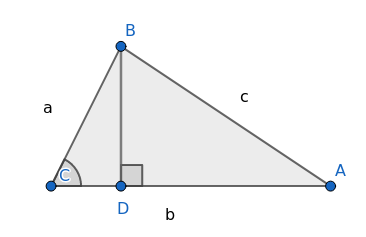
\includegraphics[width=7cm]{dot-cross-1.png}
\end{center}
\begin{center}
	Figure 1	
\end{center}
\end{minipage}

\par\noindent We can use expression (2) to derive expression (1). First, we restate expression (1) in terms of vectors. 
\newline
\newline
\begin{minipage}{.6\linewidth}		
	\begin{flalign}
		|| \vec{a} -\vec{b}||^{2} = ||\vec{a}||^{2} + ||\vec{b}||^{2} - 2 ||\vec{a}||\;||\vec{b}||\cos\theta
	\end{flalign}

		\par\noindent  We can restate the left hand side using the fact that the dot product of a vector with itself is its squared magnitude:

    \begin{flalign*}	
		|| \vec{a} - \vec{b}||^{2} = ( \vec{a} - \vec{b}) \cdot ( \vec{a} - \vec{b}) \\ 	
		= \vec{a}\cdot\vec{a} - 2(\vec{a}\cdot\vec{b}) + \vec{b}\cdot\vec{b} \\
		= ||\vec{a}||^{2}  + ||\vec{b}||^{2} - 2(\vec{a}\cdot\vec{b})
	\end{flalign*}

	\par\noindent If we compare the result we obtained on the last stem with expression 3, we see that \(2(\vec a \cdot \vec b)\) is equivalent to \(2||\vec a||  \;||\vec b|| cos \theta\):
	
		\begin{flalign*}
			||\vec{a}||^{2} + ||\vec{b}||^{2} - 2(\vec{a}\cdot\vec{b})  = ||\vec{a}||^{2} + ||\vec{b}||^{2} - 2 ||\vec{a}||\;||\vec{b}||\cos\theta  \\
			\vec{a}\cdot\vec{b} = ||\vec{a}||\;||\vec{b}||\cos\theta	
		\end{flalign*}

\end{minipage}
\begin{minipage}[c]{.4\linewidth}
	\begin{center}
		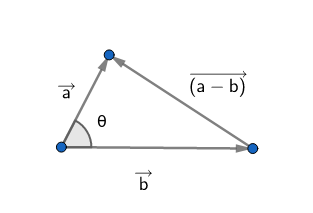
\includegraphics[width=7cm]{dot-cross-2.png}		
	\end{center}
	\begin{center}
		Figure 2	
	\end{center}
	
	
\end{minipage}
\newline
\newline
\newline
\framebox{
	\parbox{\linewidth}{
		\textbf{Ex. 4} Determine the angle between \(\vec a = <5,0>\) and \(\vec b = <-3,4>\)
		\begin{flalign*}
			\text{Since }\vec a \cdot \vec b = -15 \text{ and }
			|| \vec a || \; || \vec b|| = (5)(5) = 25 \\
			\theta = \arccos ( \frac{-15}{25}) = 2.21
		\end{flalign*}
	
	\par\noindent \textbf{ The angle between \(\vec a\) and \(\vec b\) is 2.21 radians, which is approximately \ang{126.62}}
}}

\newpage
\section {Projection}

\begin{minipage}{.6\linewidth}
	\par\noindent A useful feature of the dot product is that it assists with calculating vector projection. In Figure 2 we have the length w, which is the projection of \(\vec{a}\) onto \(\vec{b}\). We can figure out w if we know \(\theta\) and the norm of \(\vec{a}\):
	\begin{flalign*}
		w= \cos\theta ||\vec{a}|| \\	
	\end{flalign*}	

	\par\noindent Solving for \(\theta\) in expression (1) gets us \(\cos\theta=\frac{\vec{a}\cdot\vec{b}}{||\vec{a}||\;||\vec{b}||}\). Substituting this into the equation for w, we get:
	
	\begin{flalign*}
		w= \frac{\vec{a}\cdot\vec{b}\;||\vec{a}||}{||\vec{a}||\;||\vec{b}||}
	\end{flalign*}

	\begin{flalign}
		w= \frac{\vec{a}\cdot\vec{b}}{||\vec{b}||}
	\end{flalign}
\end{minipage}
\begin{minipage}[c]{.4\linewidth}
		\begin{center}
		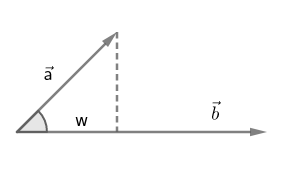
\includegraphics[width=7cm]{dot-cross-3.png}		
	\end{center}
	\begin{center}
		Figure 3	
	\end{center}
\end{minipage}
\newline
\newline
\par\noindent Expression (4) shows us how to calculate the length of a projection, but we can also derive a vector whose magnitude is equivalent to that length. Continuing with the same scenario posed by Figure 3. We first derive the unit vector for \(\vec b\), which will have a magnitude of one:
\begin{flalign*}
\hat{b} = \frac{\vec b}{ || \vec b ||} \text{}
\end{flalign*}
\par\noindent To obtain the projection vector we need to scale up \(\hat{b}\) by the projection length w, so we have:
\begin{flalign*}
\text{proj}_{b} (a) = \frac{\vec a \cdot \vec b}{ || \vec b ||} \;\;\frac{\vec b}{|| \vec b ||} = \frac{\vec a \cdot \vec b}{ || \vec b ||^2} \vec b 
\end{flalign*}
\par\noindent The square of a vector's norm is the dot product of the vector with itself, \( || \vec b ||^2 =\vec b \cdot \vec b\), so we arrive at the final form of the projection vector:
\begin{flalign}
	\text{proj}_b(a) = \frac{\vec a \cdot \vec b}{\vec b \cdot \vec b} \; \vec b
\end{flalign}

\framebox{
	\parbox{\linewidth}{

\textbf{Ex. 5} Find the projection length \(w\) of \(\vec a = <3,1>\) onto \(\vec b = <4,-2>\). Determine \(\text{proj}_b (a)\):
\newline

\begin{minipage}{.6\linewidth}

\begin{flalign*}
	w = \frac{ (3)(4) + (1)(-2) }{ \sqrt{(4)^2 + (-2)^2} } \\
	w = \frac{10}{\sqrt{20}} \\
	\text{proj}_b (a) = \frac{ (3)(4) + (1)(-2) }{ (4)(4) + (-2)(-2) } \; \vec b \\ 
	\text{proj}_b (a) = \frac{1}{2} \; <4, -2>
\end{flalign*}
\newline
\par\noindent In Figure 4, the dotted vector is \(\text{proj}b(a)\).

\end{minipage}
\begin{minipage}[c]{.4\linewidth}
	\begin{center}
		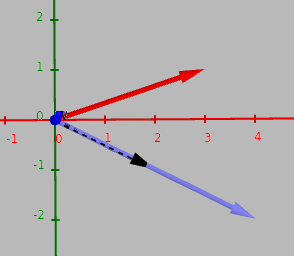
\includegraphics[width=5cm]{projected.png}		
	\end{center}
	\begin{center}
		Figure 4	
	\end{center}
\end{minipage}
}}
\newpage
\section{The Cross Product}
\par\noindent The cross product between two vectors \( \vec a\) and \( \vec b\) is denoted \(\vec a \times \vec b\). The most important aspect of the cross product is that it produces a third vector that is orthogonal to the two input vectors. 
\newline
\par\noindent The x-component of the cross product is the determinant calculated from the y and z components of the input vectors. The y-component is the determinant calculated from the x and z components. Lastly, the z-component is the determinant from the x and y components. So given \(<a_x, a_y, a_z\) and \(<b_x, b_y, b_z>\), the cross product is:
\begin{flalign}
	\vec a \times \vec b = <(a_y)(b_z) - (a_z)(b_y) , \;\; - (\;(a_x)(b_z) - (a_z)(b_x)\;), \;\; (a_x)(b_y) - (a_y) - (a_y)(b_x)>
\end{flalign}
\par\noindent We can also take the cross product of a two 2 dimensional vectors. This will simply be the determinant of a matrix comprised of the two vectors \( \vec a = <a_x, a_y>\) and \(\vec b = <b_x, b_y>\), the cross product is just: \((a_x)(b_y) - (a_y)(b_x)\). In contrast to the three dimensions case, this calculation produces a scalar.
\newline
\par \noindent We can now show that the cross product is orthogonal to both of the input vectors. If \(\vec a \times \vec b\) is orthogonal to both vectors a and b, then \( \vec{a}\cdot (\vec a \times \vec b) = 0 \) and \( \vec{b}\cdot( \vec a \times \vec b) = 0 \). We start by demonstrating this for \( \vec a\):

\begin{flalign*}
	\vec{a}\cdot(\vec a \times \vec b) \\
	= <a_{x}, a_{y}, a_{z}> \cdot <a_{y}b_{z} - a_{z}b_{y}, a_{x}b_{z} -a_{z}b_{x}, a_{x}b_{y} - a_{y}b_{x} > \\
	= a_{x}(a_{y}b_{z} - a_{z}b_{y}) - a_{y}(a_{x}b_{z} -a_{z}b_{x}) + a_{z}(a_{x}b_{y} - a_{y}b_{x}) \\
	=a_{x}a_{y}b_{z} + a_{x}a_{z}b_{y} - a_{y}a_{x}b_{z}+a_{y}a_{z}b_{x}+a_{z}a_{x}b_{y}-a_{z}a_{y}b_{x}\\
	= 0
\end{flalign*}

\par\noindent The same exercise can be done with  \( \vec b \):

\begin{flalign*}
	\vec{b}\cdot(\vec a \times \vec b) \\
	= <b_{x}, b_{y}, b_{z}> \cdot <a_{y}b_{z} - a_{z}b_{y}, a_{x}b_{z} -a_{z}b_{x}, a_{x}b_{y} - a_{y}b_{x} > \\
	= b_{x}(a_{y}b_{z} - a_{z}b_{y}) - b_{y}(a_{x}b_{z} -b_{z}b_{x}) + b_{z}(a_{x}b_{y} - b_{y}b_{x}) \\
	=b_{x}a_{y}b_{z} + b_{x}a_{z}b_{y} - b_{y}a_{x}b_{z}+b_{y}a_{z}b_{x}+b_{z}a_{x}b_{y}-b_{z}a_{y}b_{x}\\
	= 0
\end{flalign*}

\par\noindent Lastly, we want to derive the following relationship:

\begin{flalign}
	|| \vec a \times \vec b || = || \vec a || \; || \vec b || sin \theta
\end{flalign}

\par\noindent Two vectors will always be coplanar. From the perspective of the plane both vectors are located on, the z-components can be ignored for the purposes of this derivation. One way to visualize this is to suppose we are staring straight down at that plane, the same way we would look down on the xy plane. We can therefore treat \(<a_x, a_y, a_z >\) for example to be the same as \(<a_x, a_y>\).
\newline
\newline
\begin{minipage}{.6\linewidth}
	\par\noindent On the plane, we can now draw the parallelogram in Figure 5. From this, we can see that the parallelogram's area is \( || \vec a || \; || \vec b || \; sin\theta \) or the right half of Expression (7).
	\newline
	\par\noindent Since we are treating \(\vec a\) and \(\vec b\) as two dimensional vectors, its cross product is to \((a_x)(b_y) - (a_y)(b_x)\), in other words \(|| \vec a \times \vec b ||\). In the determinants chapter we saw how this is also the area of the parallelogram. 
	\newline
	\par\noindent Therefore, the area of the parallelogram is the norm of \(\vec a \times \vec b\).
\end{minipage}
\begin{minipage}[c]{.4\linewidth}
	\begin{center}
			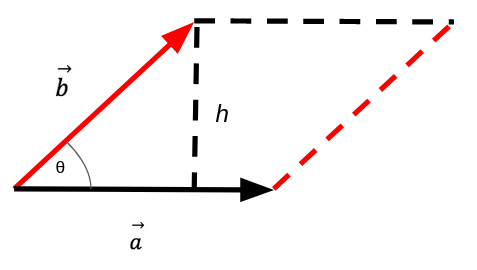
\includegraphics[width=6cm]{cross-sine.png}	
			\end{center}					\begin{center}
				Figure 5	
			\end{center}
\end{minipage}
\newpage
\framebox{
	\parbox{\linewidth}{
				\par\noindent \textbf{Ex. 6} Determine the cross product between \(\vec a = <7,2,-2>\) and \(\vec b = <-5,0,3>\).
				\newline
				\newline
				\begin{minipage}{.6\linewidth}
					
					\par\noindent x-component: \( (2)(3) - (-2)(0) = 6 \)
					\par\noindent y-component: \( -(\;(7)(3) - (-2)(-5)\; )= -11\)
					\par\noindent z-component: \( (7)(0) - (2)(-5) = 10\)
					\newline
					\begin{flalign*}
						\vec a \times \vec b = <6, -11, 10>
					\end{flalign*}
					
					
				\end{minipage}
				\begin{minipage}[c]{.4\linewidth}
					\begin{center}
						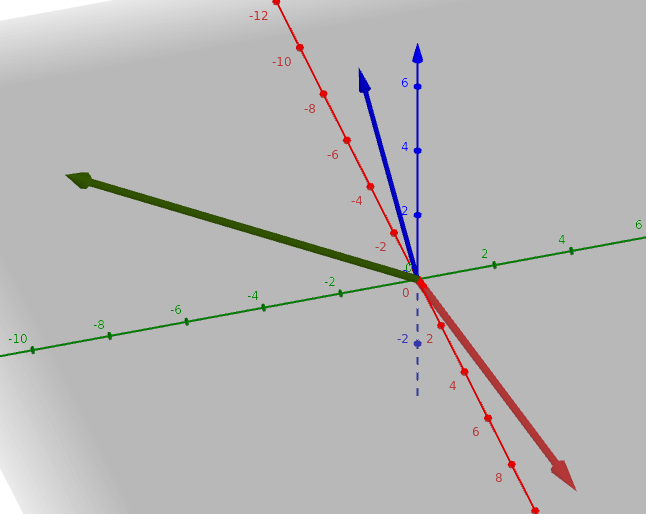
\includegraphics[width=6cm]{cross-example.png}		
					\end{center}
					\begin{center}
						Figure 6	
					\end{center}
				\end{minipage}		
			\newline
			\par \noindent In Figure 6, we have plotted \(\vec a\) in red, \(\vec b\) in blue, and the cross product in green.	
				
	}
}




\end{document}